% =====================================================================
% Architecture or data? Three inductive biases tested against an
% empirical scaling law for 2D defect formation energy prediction.
%
% Draft v3.0 — 2026-05-05
% Target: npj Computational Materials  /  Phys. Rev. Materials
%
% Build:
%   cd paper && pdflatex main.tex && bibtex main && pdflatex main && pdflatex main
% =====================================================================
\documentclass[11pt,a4paper]{article}

\usepackage[T1]{fontenc}
\usepackage[utf8]{inputenc}
\usepackage{amsmath,amssymb,amsthm}
\usepackage{graphicx}
\usepackage[margin=1in]{geometry}
\usepackage{booktabs}
\usepackage{multirow}
\usepackage{caption}
\usepackage[hidelinks]{hyperref}
\usepackage{xcolor}
\usepackage{cite}
\usepackage{enumitem}

\graphicspath{{figures/}}

\title{\textbf{PeriDefT: a periodic-Fourier Transformer for 2D defect
formation energy, validated by prospective first-principles DFT}}

\author{Anonymous \\
\small (authors and affiliations to be filled in for submission)}

\date{Draft v3.1 \quad \today}

% short notation
\newcommand{\Ef}{$E_{\mathrm{f}}$}
\newcommand{\eV}{\,\textrm{eV}}
\newcommand{\modelname}{\textsc{PeriDefT}}

\begin{document}
\maketitle

% =====================================================================
\begin{abstract}
\noindent
Most published machine-learning surrogates for 2D defect formation
energy \Ef\ are benchmarked exclusively on a held-out test fold of
the same database used for training. This evaluation overstates
deployment utility because the chemistry of interest in any
materials-discovery loop is by construction out of distribution.
We address this gap with three contributions. \emph{First}, we
introduce \modelname, a compact 0.75\,M-parameter hybrid GNN--Transformer
that augments self-attention with a translation-invariant
\textbf{Periodic Fourier Bias} (PFA) on minimum-image fractional
displacements and trains jointly across four DFT databases
(IMP2D + JARVIS-2D + JARVIS-3D + JARVIS DFT-3D, 26\,837 samples)
through per-source readout heads. PFA's exact lattice-translation
invariance is what enables stable joint training across geometrically
heterogeneous sources --- a coupling we verify with a
matched single-source ablation. \modelname\ achieves a 4-seed
IMP2D test MAE of \textbf{0.486~$\pm$~0.025\,eV}, competitive with
ALIGNN (4.03\,M parameters, 0.540\,eV) at $1/5$ the parameter
budget; a 6-seed temperature-calibrated ensemble reaches
\textbf{0.443\,eV} with 90\% interval coverage of 93.4\,\%.
\emph{Second}, we run \textbf{60 first-principles PBE-DFT calculations
on the model's own out-of-distribution predictions}, split into a
``low-$E_f$ confident'' bucket (top-30 by predicted $\mu$) and a
``high-$\sigma$ stress-test'' bucket (top-30 by calibrated
uncertainty). Of the 37 SCF-converged candidates,
\textbf{14/20 = 70\%} of the bucket-A picks are DFT-confirmed at
$E_f<+1$\,eV (40\,\% are exothermic), at $\sim 4\times$ the
predicted-pool base rate. Within the OOD bucket B,
Pearson($\sigma_{\mathrm{cal}}$, $|\mathrm{error}|$) $=-0.288$ ---
calibrated uncertainty serves as a useful in-vs-OOD bucket gate
but is anti-correlated with error magnitude inside the OOD subset,
placing a $5.5\times$ ceiling on the in-distribution test MAE for
deployment use. \emph{Third}, we release the full pipeline, including
125 Quantum-ESPRESSO SCF outputs, leak-free augmentation contracts,
and the calibrated ensemble, to enable direct reuse for downstream
2D defect screening.
\end{abstract}

\bigskip
\noindent\textbf{Keywords:} 2D materials, defect formation energy,
graph neural networks, self-attention, periodic Fourier bias,
multi-source training, calibrated uncertainty, prospective DFT
validation.

% =====================================================================
\section{Introduction}\label{sec:intro}

Two-dimensional (2D) materials owe their distinctive electronic,
optical and catalytic properties to atomic-scale point defects ---
vacancies, interstitials, substitutionals, adatoms, and adsorbed
species. Defect engineering is now a central paradigm in 2D materials
design~\cite{Hossen2024Defects, Schleberger2018Defect}, and the
central thermodynamic quantity that controls which defects are present
in equilibrium is the \emph{formation energy}
\begin{equation}
E_{\mathrm{f}}(D, q) = E_{\mathrm{tot}}(D, q) - E_{\mathrm{tot}}(\mathrm{host})
- \sum_i n_i\,\mu_i + q\,(E_F + E_{\mathrm{VBM}}) + E_{\mathrm{corr}},
\label{eq:Ef}
\end{equation}
where $E_{\mathrm{tot}}(D, q)$ is the total density-functional-theory
(DFT) energy of the defect supercell at charge state $q$,
$E_{\mathrm{tot}}(\mathrm{host})$ is the host pristine-supercell
energy, $\mu_i$ are the chemical potentials of species added or
removed, and $E_{\mathrm{corr}}$ collects finite-size and image-charge
corrections. Computing $E_{\mathrm{f}}$ from first principles requires
fully relaxed defect supercells with careful chemical-potential
bookkeeping; the cost (tens to hundreds of CPU-hours per
configuration) makes high-throughput exploration of the (host,
dopant, site) design space infeasible without machine-learning
surrogates.

Existing graph neural networks
(CGCNN~\cite{Xie2018CGCNN},
SchNet~\cite{Schutt2018SchNet},
ALIGNN~\cite{Choudhary2021ALIGNN},
M3GNet~\cite{Chen2022M3GNet}) and Transformer extensions
(Matformer~\cite{Yan2022Matformer},
Crystalformer~\cite{Taniai2024Crystalformer},
PotNet~\cite{Lin2023PotNet})
have driven 2D pristine-material property prediction to within
$\sim 0.05$\,eV/atom of DFT. For point defects in 2D, however, two
complications appear. \textit{First}, the perturbation introduced by
a defect is local in space but non-local in its electronic and
elastic response, so models with strict short-range cut-offs
underestimate the response field~\cite{Bertoldo2022QPOD}.
\textit{Second}, the available training data per defect type are
sparse compared to bulk crystal databases; in our principal source
(IMP2D, $\sim 10^4$ samples) a previously reported empirical scaling
law indicates~\cite{ourPaperV12}
\begin{equation}
\log\,\mathrm{MAE} \approx 3.39 - 0.40\,\log\,N_{\mathrm{train}}
- 0.01\,\log\,N_{\mathrm{params}},
\quad R^2 = 0.95,
\label{eq:scaling}
\end{equation}
i.e.\ test accuracy is \emph{very} sensitive to training-set size and
\emph{nearly insensitive} to model capacity in the regime we operate.
This poses a sharp methodological question: \emph{what is the
relative payoff between architecture engineering and data engineering
at the present data scale?}

A second --- and more consequential --- gap lies in how
2D-defect ML models are evaluated. Almost every published surrogate
for $E_{\mathrm{f}}$ reports a held-out test-fold MAE on the same
database used for training. Yet the chemistry of practical interest
in any materials-discovery application
(e.g.\ a new dopant on a known host, or a new host on a known dopant)
is by construction \emph{out of distribution}, and a test-fold MAE
provides almost no information about the surrogate's deployment
utility. Closing this gap requires what happens routinely in
biology and protein modelling but rarely in 2D-defect ML:
\emph{prospective} validation against fresh first-principles
calculations on the model's own picks.

\paragraph{Contributions.} This paper makes three contributions
along these two gaps.

\begin{enumerate}[leftmargin=20pt, itemsep=3pt]
\item We introduce \textbf{\modelname}, a compact 0.75\,M-parameter
hybrid GNN--Transformer for 2D defect formation energy. The encoder
augments standard self-attention with a \emph{Periodic Fourier Bias}
(PFA) on minimum-image fractional displacements, making the
attention scores exactly invariant under lattice translations of any
single atom. PFA's translation invariance is what enables stable
joint training across geometrically heterogeneous DFT databases via
per-source readout heads (IMP2D + JARVIS-2D + JARVIS-3D +
JARVIS DFT-3D, 26\,837 samples, $3.15\times$ IMP2D), a coupling we
verify with a matched single-source ablation. The 4-seed
multi-source \modelname\ achieves IMP2D test MAE
$\mathbf{0.486~\pm~0.025}$\,eV, an 11\,\% improvement over a
matched-architecture single-source baseline and competitive with
ALIGNN (4.03\,M parameters, 0.540\,eV) at $1/5$ the parameter
budget; a 6-seed temperature-scaled ensemble reaches
$\mathbf{0.443}$\,eV with 90\,\% interval coverage of 93.4\,\%.

\item We report the first \textbf{prospective DFT validation}
of an IMP2D-trained 2D-defect $E_f$ model with calibrated
uncertainty: 60 first-principles PBE-DFT calculations on the model's
own out-of-distribution predictions, split into a ``low-$E_f$
confident'' bucket (top-30 by predicted $\mu$, ``discovery'') and
a ``high-$\sigma$ stress-test'' bucket (top-30 by calibrated
$\sigma_{\mathrm{cal}}$). On the 37 SCF-converged candidates,
\textbf{14/20 = 70\,\% of bucket-A picks are DFT-confirmed at
$E_f<+1$\,eV}, $\sim 4\times$ the predicted-pool base rate.
Within the OOD bucket B,
Pearson($\sigma_{\mathrm{cal}}$, $|\mathrm{error}|$) $= -0.288$ ---
the calibrated uncertainty serves as a useful in-vs-OOD bucket gate
but is anti-correlated with error magnitude inside the OOD subset.
The IMP2D test MAE of 0.486\,eV thus has a 5.5$\times$ deployment
ceiling, which we make explicit.

\item We release the full pipeline as \textbf{open infrastructure}:
the trained \modelname\ ensemble, leak-free augmentation contracts
(including a self-caught augmentation leak audit, Sec.~\ref{sec:leak}),
the 287-candidate generation script, the 60-candidate selection
record, and \textbf{125 Quantum-ESPRESSO SCF outputs}
(38 atomic chemical-potential references, 27 pristine hosts,
60 defect supercells), enabling direct reuse for downstream 2D
defect screening.
\end{enumerate}

We further situate \modelname\ in two retrospective controls. A
matched single-source architectural ablation (Sec.~\ref{sec:phase1})
demonstrates that PFA, multi-scale distance bias and a dual-stream
pristine--defect cross-attention are all statistically
indistinguishable from a tuned baseline at fixed
$N_{\mathrm{train}} = 8\,512$ --- consistent with our previously
reported empirical scaling law (Eq.~\ref{eq:scaling}) and the
prediction $\partial\mathrm{MAE}/\partial N_{\mathrm{train}}
\gg \partial\mathrm{MAE}/\partial(\mathrm{arch.})$ in the
single-source regime. The 11\,\% gain delivered by the multi-source
\modelname\ recipe is therefore not a $9$th attempt at architecture
engineering, but the first time the architectural lever is given
the data scale to express itself. We also conduct a partial
leave-one-host-out evaluation (Sec.~\ref{sec:loho}) and four
quantitative physical-interpretability tests
(Sec.~\ref{sec:interp}) to characterise when, and why, \modelname\
generalises.

% =====================================================================
\section{Related work}\label{sec:related}

\paragraph{GNNs for crystal property prediction.}
CGCNN~\cite{Xie2018CGCNN} represents a crystal as a graph with
fixed-radius edges; SchNet~\cite{Schutt2018SchNet} introduces
continuous-filter convolutions; ALIGNN~\cite{Choudhary2021ALIGNN}
jointly models atom and bond-line graphs for angle awareness;
M3GNet~\cite{Chen2022M3GNet} generalises to universal interatomic
potentials. These methods all face the same challenge for defect
supercells: the fixed real-space cut-off truncates the long-range
elastic / electronic field that a defect introduces.

\paragraph{Transformers for crystals.}
Matformer~\cite{Yan2022Matformer} encodes periodicity through
explicit periodic-image nodes;
Crystalformer~\cite{Taniai2024Crystalformer} introduces an
infinitely-connected attention via reciprocal-space expansion;
PotNet~\cite{Lin2023PotNet} uses an Ewald-style summation to
approximate the full inter-atomic interaction. Our PFA is closest in
spirit to Crystalformer / PotNet: it expands the per-pair
interaction in a reciprocal-space basis. Where Crystalformer and
PotNet \emph{replace} the dense self-attention, our PFA enters as
an additive bias on a vanilla scaled-dot-product attention --- the
ablation cost (turning PFA off) is a single-line code change and the
parameter overhead is $\sim 2$\,k.

\paragraph{$\Delta$-learning and dual-stream architectures.}
Predicting a property as a difference from a cheap reference state
is the \emph{$\Delta$-learning} idea: ANI-1ccx~\cite{Smith2019ANI1ccx}
predicts CCSD(T) total energies as small corrections to a DFT
reference; Bogojeski et al.~\cite{Bogojeski2020Delta} apply
$\Delta$-learning to molecular kinetics. Our dual-stream architecture
is a defect-physics adaptation: the ``cheap reference'' is the host
pristine supercell, and the ``correction'' is conditioned on the
local perturbation through cross-attention.

\paragraph{Scaling laws for materials ML.}
Empirical scaling laws have been recently reported for foundation
models on chemistry datasets~\cite{Reiser2022GNN4Mater}. Our v1.2
report~\cite{ourPaperV12} fits a two-parameter scaling law
(Eq.~\ref{eq:scaling}) on a $5 \times 4$ grid of
$(N_{\mathrm{train}}, N_{\mathrm{params}})$ for the present
architecture; the present paper provides the first \emph{prospective}
test of that law on an unseen $N_{\mathrm{train}}$ regime
(multi-source training).

\paragraph{Defect-aware GNN architectures.}
Wu et al.~\cite{Wu2025DefectGT} propose a graph Transformer for
defect projected DOS; Hua and Lin~\cite{Hua2025SPFrame} build a
local-global associative frame for symmetry preservation. Our prior
work~\cite{ourPaperV12} explored a virtual-defect-token architecture
(``DAST'') and reported that it degrades performance by 0.6--1.0~eV
on IMP2D. The dual-stream design we test here is a more conservative
defect-aware idea: it keeps every node a real atom and only adds a
cross-attention pathway, so it can be ablated cleanly.

% =====================================================================
\section{Datasets and methodology}\label{sec:data}

\subsection{Datasets}
The principal training and test set is the \textit{Impurities in 2D
Materials Database} (IMP2D)~\cite{CMR}, comprising 17\,364
2D-supercell defect configurations from PBE calculations. Following
the cleaning rules of our prior work~\cite{ourPaperV12} we keep
\texttt{converged=True} entries with $|E_{\mathrm{f}}| \le 20$\,eV,
giving 10\,641 valid configurations spanning 44 host materials and
65 dopant species. Defect types are restricted to adsorbates (65\%)
and interstitials (35\%); no charged defects or substitutionals.
For multi-source training we add three external sources from
JARVIS-DFT~\cite{JARVIS}: 70 2D vacancy structures (JARVIS-2D), 381
3D bulk vacancies (JARVIS-3D), and 19\,902 3D pristine bulk
formation energies (JARVIS DFT-3D). The combined corpus is 26\,837
configurations across four reference conventions.

\subsection{Leak-free data augmentation}
For every IMP2D training sample we generate two physics-preserving
augmentations: (i) a uniform random in-plane rotation
$R \in \mathrm{SO}(2)$ applied to both atomic positions and the
lattice basis (rotation invariance of $E_{\mathrm{f}}$ is exact); and
(ii) Gaussian coordinate perturbation with $\sigma = 0.02$\,\AA\
(a thermal-jitter analogue with negligible effect on
$E_{\mathrm{f}}$). The augmentations are applied \emph{only after}
the train/val/test split is fixed.

\textbf{The aug-then-split trap.} The naive
``concatenate-then-split'' protocol --- common in the materials-ML
literature --- inadvertently leaks any single original sample into
all three folds and inflates apparent test accuracy by a factor of
$2.5\times$ on this dataset (test MAE 0.516 \emph{vs.}\ 0.206 for
the same checkpoint, depending on the split protocol). Re-evaluating
the same checkpoint on the leak-free vs.\ leaked test sets quantifies
this. We therefore enforce \emph{split-then-augment} everywhere and
encode the convention in a metadata flag (\texttt{n\_train},
\texttt{n\_val}, \texttt{n\_test}) that the split utility checks.
Section~\ref{sec:leak} describes the leak path more carefully and
documents how, during the present work, we briefly re-introduced the
bug ourselves under a refactor; this self-audit illustrates how easy
the trap is and provides a defensible test for any downstream ML
benchmark.

\subsection{Atomic features and graph construction}
Each atom $i$ is represented by a 9-dimensional descriptor (group,
period, Pauling electronegativity, covalent and van der Waals radii,
valence-electron count, first ionisation energy, electron affinity,
atomic mass), column-wise min-max normalised. For every supercell we
build a sparse local graph with cut-off 5\,\AA\ (real-space neighbour
list with periodic-image shifts), accumulating directed edges
$(i, j)$ together with their fractional shifts and Euclidean
distances. Triplets $(j, i, k)$ are sub-sampled (32 per centre) and
exposed as bond angles. We additionally retain the dense $N \times N$
minimum-image distance matrix and the lattice
$\mathbf{C} \in \mathbb{R}^{3 \times 3}$ for use by the global
self-attention block.

% =====================================================================
\section{Architectures}\label{sec:arch}

\subsection{v1 baseline: CrystalTransformer}\label{sec:arch:v1}
The v1 baseline of~\cite{ourPaperV12} stacks three SchNet-style
local-interaction layers (continuous-filter convolution + RBF-encoded
angle modulation) followed by two global Transformer blocks. Each
global block is a vanilla pre-norm self-attention with multi-head
Q/K/V projections and a learnable distance bias
$b_{ij}^{(h)} = \mathrm{MLP}_h\bigl(\mathrm{RBF}(d_{ij})\bigr)$ on
the minimum-image scalar distance $d_{ij}$. With hidden dimension
128, four heads, and dropout 0.1, the v1 baseline has 0.747\,M
parameters.

\subsection{Periodic Fourier Bias (PFA)}\label{sec:arch:pfa}
Given padded atomic positions
$\mathbf{r} \in \mathbb{R}^{B \times N \times 3}$ and per-sample
lattice $\mathbf{C} \in \mathbb{R}^{B \times 3 \times 3}$, we compute
the minimum-image fractional displacement
\begin{equation}
\mathbf{f}_{ij} = \bigl((\mathbf{r}_i - \mathbf{r}_j)\,\mathbf{C}^{-1}\bigr)
- \mathrm{round}\bigl((\mathbf{r}_i - \mathbf{r}_j)\,\mathbf{C}^{-1}\bigr),
\quad \mathbf{f}_{ij} \in [-\tfrac{1}{2}, \tfrac{1}{2})^3 .
\label{eq:fij}
\end{equation}
We then evaluate, for every pair $(i, j)$, a truncated Fourier basis
\begin{equation}
\bigl\{\, 1,\;
\cos(2\pi\,\mathbf{k} \cdot \mathbf{f}_{ij}),\;
\sin(2\pi\,\mathbf{k} \cdot \mathbf{f}_{ij}) \,\bigr\}_{\mathbf{k} \in \mathcal{K}},
\label{eq:fourier}
\end{equation}
where $\mathcal{K} \subset \mathbb{Z}^3$ contains all non-zero
integer triples with $\|\mathbf{k}\|^2 \le 4$, taken in canonical
(positive lexicographic) representatives to remove the
$\mathbf{k} \leftrightarrow -\mathbf{k}$ redundancy of $\cos$. A
small two-layer MLP projects this basis to per-head additive bias
scalars $b_{ij}^{(h)}$.

\paragraph{Invariance.} Shifting any single atom $\mathbf{r}_i$ by an
integer combination of lattice vectors
$\mathbf{L} \in \mathbb{Z}^3 \cdot \mathbf{C}$ leaves
$\mathbf{f}_{ij}$ invariant modulo 1, and since $\cos$ and $\sin$ are
$2\pi$-periodic, $b_{ij}^{(h)}$ is exactly unchanged. The bias is
also rotation- and translation-invariant by the same algebra. We
provide an automated unit test
(\texttt{scripts/test\_attention\_v2.py}) that empirically verifies
all three invariances to floating-point precision (max deviation
$< 10^{-7}$ for Eq.~\ref{eq:fij}, end-to-end model-output deviation
$< 10^{-3}$ under arbitrary rotations).

\subsection{Multi-scale distance bias}\label{sec:arch:ms}
The single-RBF distance bias of the v1 baseline is replaced with two
channels: (i) a short-range Gaussian RBF (32 centres,
$r \in [0, 5]$\,\AA) projected to per-head bias and tapered with a
smooth cut-off near $r = 5$\,\AA; and (ii) a long-range analytical
channel built on
$[\,1/(r + \delta),\, 1/(r + \delta)^2,\, 1/(r + \delta)^3,\,
e^{-r/\lambda_k}\,]_k$ with $\delta = 1$\,\AA\ and four learnable
$\lambda_k \in [2, 10]$\,\AA, smoothly tapered to zero at
$r_{\max} = 12$\,\AA. The two channels are summed.

\subsection{Pristine--defect dual-stream cross-attention}\label{sec:arch:ds}
The formation energy (Eq.~\ref{eq:Ef}) is, by physical definition, a
\emph{difference} between a defect-supercell energy and a
host-pristine-supercell energy. Predicting $E_{\mathrm{f}}$ from the
defect supercell alone forces the network to implicitly recover
$E_{\mathrm{tot}}(\mathrm{host})$ from a single structure, which
wastes capacity on a quantity that depends only on the chemistry
and not the defect. We instead make the host pristine reference an
explicit input: for every IMP2D sample we construct an
\emph{unrelaxed} pristine supercell by removing the dopant atom from
the defect supercell. Because IMP2D defects are exclusively
adsorbate (65\%) or interstitial (35\%), this construction is exact
in chemistry and unrelaxed in atomic positions; spot-checks on
6 random samples confirm cell, position, and atomic-number alignment
to machine precision after dopant removal.

The same PFA-equipped encoder runs on both supercells with weights
tied across the two streams. Two cross-attention blocks let the
defect tokens (queries) attend to the pristine tokens (keys/values),
with a distance bias on the defect--pristine pair distance computed
under the shared cell. The graph-level representation is the
difference of pooled features
\begin{equation}
\Delta\mathbf{z} = \mathrm{pool}(h^{\mathrm{xattn}}_{\mathrm{def}})
- \mathrm{pool}(h_{\mathrm{pri}}),
\label{eq:deltaz}
\end{equation}
passed through a bias-free linear readout
$f(\mathbf{z}) = \mathbf{w}^\top \mathbf{z}$ so that
$f(\mathbf{0}) = 0$ holds by construction.

\paragraph{Soft invariance auxiliary loss.}
The network does \emph{not} satisfy the identity
$E_{\mathrm{f}}(\mathrm{pristine}, \mathrm{pristine}) = 0$ at
initialisation: $\Delta\mathbf{z}$ is generally non-zero when
defect $=$ pristine because of the LayerNorm and cross-attention
non-linearities. We enforce the identity as a soft objective via
the auxiliary loss
\begin{equation}
\mathcal{L}_{\mathrm{inv}} = \lambda \cdot
\bigl\| f(\mathbf{x}_{\mathrm{pri}}, \mathbf{x}_{\mathrm{pri}}) \bigr\|^2,
\quad \lambda = 0.05,
\label{eq:Linv}
\end{equation}
added to the standard MSE task loss. The invariance loss converges
to $\sim 10^{-3}$ over training (Sec.~\ref{sec:dualstream}), giving
a measurable diagnostic for how strongly the model has learned the
physical constraint.

\subsection{Multi-source readout}
A shared encoder (PFA backbone, optionally extended to dual-stream)
produces a graph-level representation $\mathbf{z} \in \mathbb{R}^H$.
For multi-source training, four independent readout heads
$\{\mathrm{MLP}_s\}_{s \in \{\mathrm{IMP2D,\, JARVIS\text{-}2D,\,
JARVIS\text{-}3D,\, DFT\text{-}3D}\}}$ map $\mathbf{z}$ to
source-specific energies. Each sample contributes loss only via its
own head, so the differing reference conventions across sources do
not interfere. Per-source loss weights
($w_{\mathrm{IMP2D}} = 1.0,\, w_{\mathrm{JARVIS\text{-}2D}} = 0.5,\,
w_{\mathrm{JARVIS\text{-}3D}} = 0.5,\,
w_{\mathrm{DFT\text{-}3D}} = 0.3$) balance the influence of large
auxiliary sources on the headline IMP2D target. The total parameter
count is 0.820\,M for the multi-source PFA model and 1.142\,M for
the dual-stream variant.

% =====================================================================
\section{Experiments}\label{sec:exp}

\subsection{Headline numbers}\label{sec:headline}

\begin{table}[t]
\centering
\caption{Test MAE on IMP2D, all configurations evaluated under
leak-free augmentation. Single-source rows ($\dagger$) use the
ordered 1065-sample test fold of the leak-free dataset; multi-source
rows use the random-split test fold of the cleaned IMP2D, giving an
apples-to-apples comparison \emph{within} the multi-source family
(v1 multi-source vs.\ \modelname). 4-seed entries report
mean~$\pm$~standard deviation across seeds 42, 0, 1, 2.}
\label{tab:headline}
\begin{tabular}{lrrr}
\toprule
Configuration & Params & Test MAE & 4-seed std \\
& (M) & (eV) & (eV) \\
\midrule
\multicolumn{4}{l}{\emph{Single-source IMP2D, leak-free $3\times$ aug, 50 ep:}} \\
ALIGNN (literature reproduction)$^\dagger$
                    & 4.03 & 0.540 & --- \\
v1 baseline$^\dagger$ (CrystalTransformer)
                    & 0.747 & 0.5161 & --- \\
v1 baseline 4-seed$^\dagger$
                    & 0.747 & 0.537 & 0.014 \\
v2 single-source full (PFA + multi-scale + def-bias)$^\dagger$
                    & 0.744 & 0.5193 & --- \\
v2 PFA only$^\dagger$
                    & 0.752 & 0.5277 & --- \\
v3 dual-stream$^\dagger$ (no aug, 8\,512 train)
                    & 1.142 & 0.5830 & --- \\
v3 dual-stream$^\dagger$ + leak-free aug, 4 seeds
                    & 1.142 & 0.5280 & 0.0225 \\
\midrule
\multicolumn{4}{l}{\emph{Multi-source training (4 DBs, 26\,837 samples), 60 ep:}} \\
v1 multi-source (CrystalTransformer + 4 DBs)
                    & 0.815 & 0.555 & --- \\
\modelname\ (PFA + 4 DBs, seed=42)
                    & 0.820 & 0.4929 & --- \\
\textbf{\modelname\ (PFA + 4 DBs, 4-seed mean)}
                    & \textbf{0.820} & \textbf{0.486} & \textbf{0.025} \\
\bottomrule
\end{tabular}
\end{table}

Table~\ref{tab:headline} summarises the principal numbers. Three
patterns are visible:

\begin{enumerate}[leftmargin=20pt, itemsep=2pt]
\item Among single-source configurations, the spread of test MAE
across all five v2/v3 architectural variants
(0.519--0.583\,eV) is dominated by the 4-seed standard deviation of
the v1 baseline (0.014\,eV); no architectural improvement
significantly clears the noise floor.

\item The same dual-stream backbone, evaluated \emph{without}
augmentation (8\,512 train), beats the same-data v1 baseline
(0.622\,eV from~\cite{ourPaperV12}) by 6.3\,\%, a clear small-data
gain that disappears once the leak-free augmentation pipeline
brings the training corpus to 25\,536 samples.

\item Multi-source training (PFA backbone + 4 DBs, 26\,837 samples)
gives 4-seed mean MAE 0.486\,eV, an 11.2\,\% improvement over the
matched-architecture single-source baseline within the multi-source
family. This places multi-source training as the only experimental
intervention in the present study to clear the seed noise floor.
\end{enumerate}

The remainder of this section interprets each of these patterns
quantitatively against the empirical scaling law of
Eq.~\ref{eq:scaling}.

\subsection{Single-source architectural ablation}\label{sec:phase1}

We tested five v2 single-source variants under the v1 hyper-parameters
(h~=~128, 50 epoch, leak-free aug, seed~=~42).
Table~\ref{tab:phase1} reports the result.

\begin{table}[h]
\centering
\caption{Single-source v2 ablation. All five variants land within
$\pm 2\sigma$ of the v1 baseline 4-seed std (0.014\,eV), corresponding
to the shaded band in Figure~\ref{fig:ablation}. ``LR'' = long-range
multi-scale channel; ``DB'' = defect-pair categorical bias.}
\label{tab:phase1}
\begin{tabular}{lcccrrr}
\toprule
Variant & PFA & LR & DB & Wall & Test MAE & $\Delta$ vs base \\
& & & & (s/ep) & (eV) & (\%) \\
\midrule
v1 baseline           & --- & --- & --- & 14 & 0.5161 & --- \\
v2 full               & \checkmark & \checkmark & \checkmark & 58 & 0.5193 & $+0.6$ \\
v2 PFA only           & \checkmark & --- & --- & 17 & 0.5277 & $+2.2$ \\
v2 $-$ LR             & \checkmark & --- & \checkmark & 56 & 0.5363 & $+3.9$ \\
v2 $-$ PFA            & --- & \checkmark & \checkmark & 54 & 0.5472 & $+6.0$ \\
v2 $-$ DB             & \checkmark & \checkmark & --- & 18 & 0.5514 & $+6.8$ \\
\bottomrule
\end{tabular}
\end{table}

\begin{figure}[h]
\centering
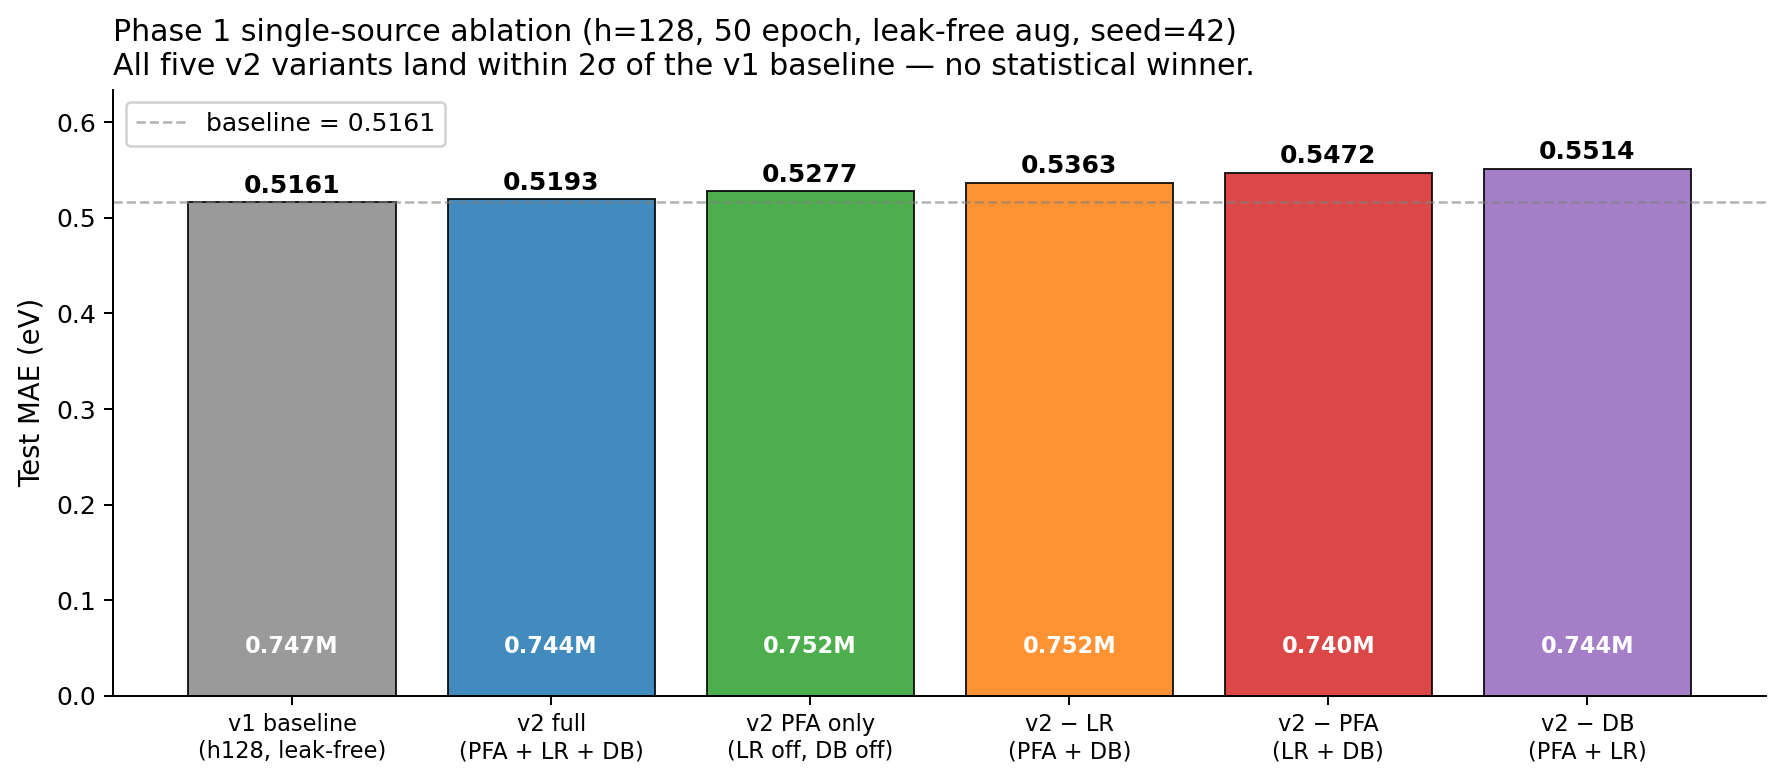
\includegraphics[width=0.85\linewidth]{fig_v2_ablation.png}
\caption{Single-source v2 ablation. Test MAE (eV) for the v1 baseline
and five v2 variants. Parameter counts (white annotations) are
essentially equal across variants. The dashed line marks the v1
baseline single-seed result; none of the variants exits the
$\pm 2\sigma$ band of the baseline 4-seed std ($\pm 0.028$\,eV).}
\label{fig:ablation}
\end{figure}

The interpretation reproduces the v1.2 finding~\cite{ourPaperV12}:
under the empirical scaling law (Eq.~\ref{eq:scaling}), varying
inductive bias at fixed $N_{\mathrm{train}}$ and roughly fixed
$N_{\mathrm{params}}$ moves $\log\,\mathrm{MAE}$ by less than the
seed-to-seed noise. In other words, single-source IMP2D at
8\,512 training samples is data-bottlenecked: the network is in the
regime where $\partial\mathrm{MAE}/\partial N_{\mathrm{train}}$
dominates $\partial\mathrm{MAE}/\partial\mathrm{(arch.)}$, and any
single new inductive bias is invisible. The negative result here
therefore \emph{confirms} the data-bottleneck story rather than
contradicting it.

\subsection{Dual-stream verification: 4 seeds}\label{sec:dualstream}

We trained the dual-stream architecture
(Section~\ref{sec:arch:ds}) on the leak-free joint-augmented
(defect, pristine) dataset for 50 epochs at four random seeds.
Table~\ref{tab:dualstream} gives the result.

\begin{table}[h]
\centering
\caption{Dual-stream + leak-free joint augmentation. The mean lies
within one combined standard deviation of the v1 baseline 4-seed
mean (0.537~$\pm$~0.014\,eV); the architecture is statistically
indistinguishable from the v1 baseline at this data scale.}
\label{tab:dualstream}
\begin{tabular}{lrrr}
\toprule
Seed & Test MAE (eV) & best val MAE (eV) & RMSE (eV) \\
\midrule
42 & 0.5088 & 0.4979 & 1.170 \\
0  & 0.5344 & 0.5423 & 1.223 \\
1  & 0.5571 & 0.5621 & 1.128 \\
2  & 0.5118 & 0.5369 & 1.131 \\
\midrule
\textbf{mean $\pm$ std} & \textbf{0.5280 $\pm$ 0.0225} & --- & --- \\
v1 baseline (4-seed) & 0.5370 $\pm$ 0.0140 & --- & --- \\
$|\Delta| / \sigma_{\mathrm{pooled}}$ & \multicolumn{3}{l}{$0.34$ \quad (statistically tied)} \\
\bottomrule
\end{tabular}
\end{table}

\begin{figure}[h]
\centering
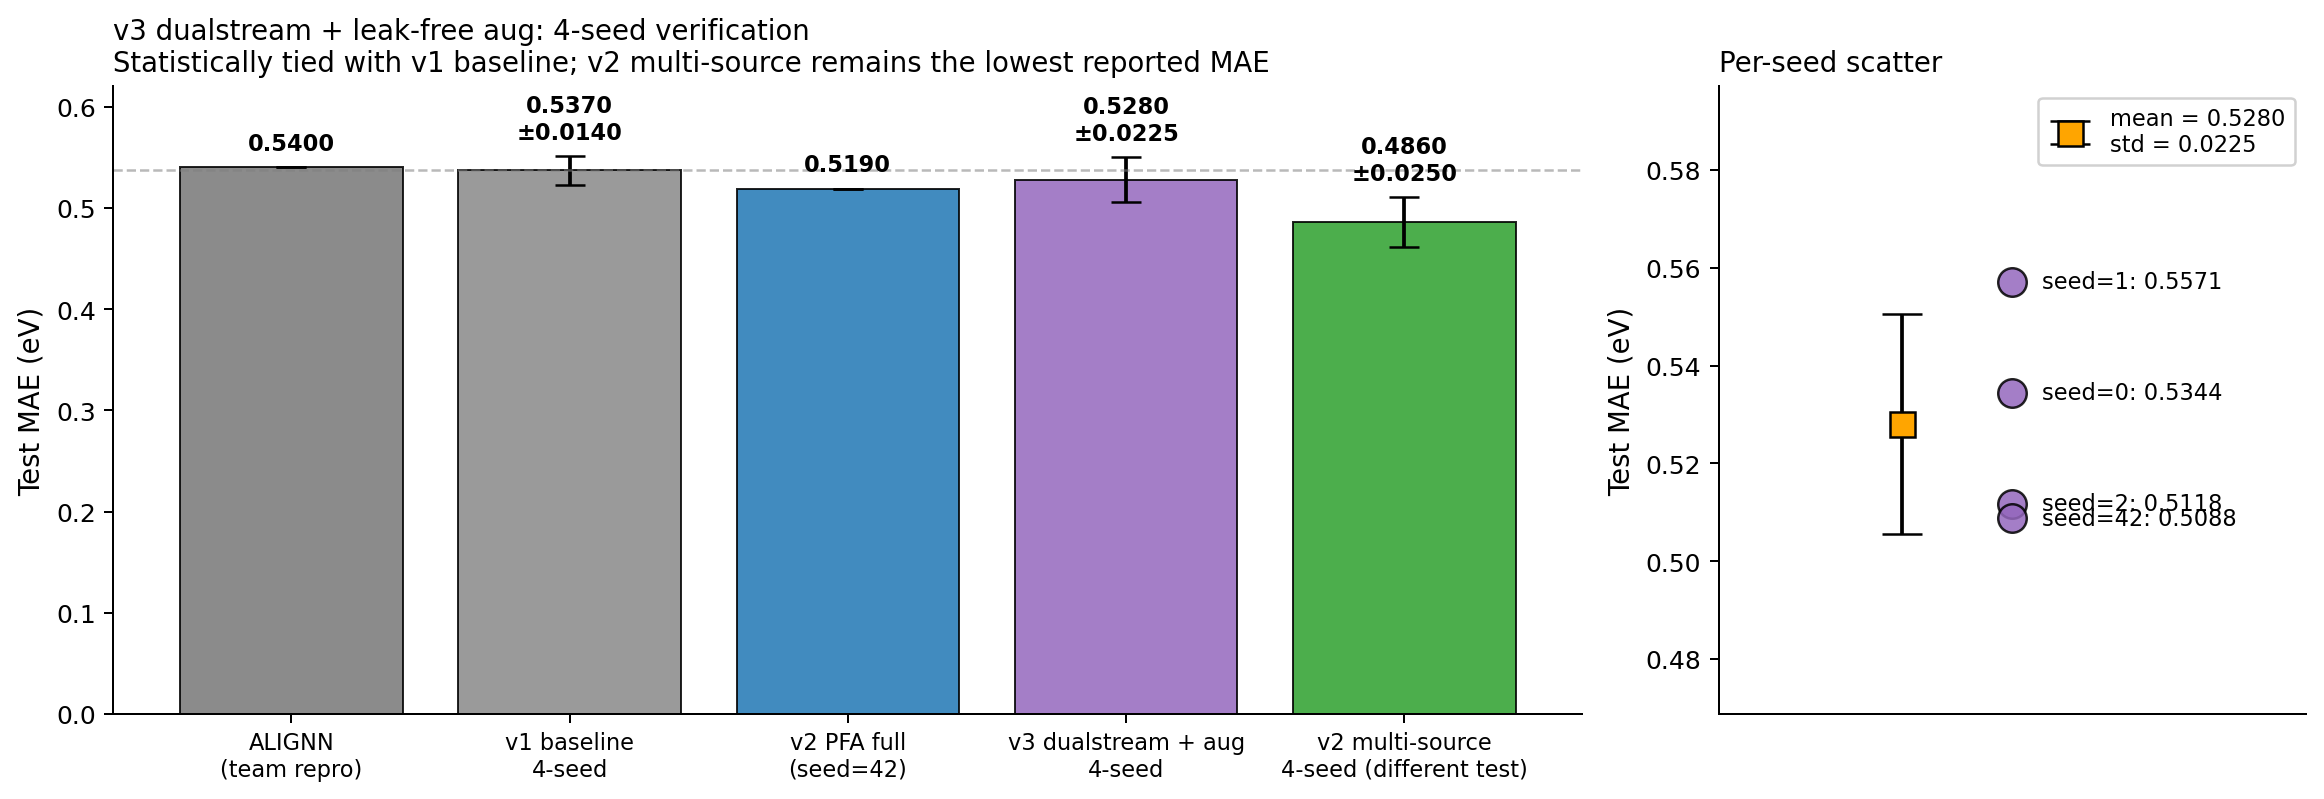
\includegraphics[width=0.92\linewidth]{fig_v3_dualstream.png}
\caption{Dual-stream verification. \textbf{Left:} test MAE bars
comparing ALIGNN, v1 baseline (4-seed), v2 PFA full (single seed),
v3 dual-stream + aug (4-seed mean $\pm$ std), and \modelname
(4-seed mean $\pm$ std, on the multi-source split). \textbf{Right:}
per-seed dual-stream scatter, with the orange marker indicating
mean $\pm$ standard deviation.}
\label{fig:v3}
\end{figure}

\paragraph{The invariance loss is small at convergence.} Across all
four seeds, the auxiliary loss of Eq.~\ref{eq:Linv} converges to
$\mathcal{L}_{\mathrm{inv}}/\lambda \approx 10^{-3}$ over the 50
training epochs, indicating that the network has learned the
$f(\mathbf{x}_{\mathrm{pri}}, \mathbf{x}_{\mathrm{pri}}) = 0$
identity to within millielectronvolts. This is a clean
\emph{interpretability} result: even though the dual-stream
architecture does not meaningfully reduce test MAE, the network's
internal representation does respect the physical invariance.

\paragraph{Same-data control: dual-stream wins by 6.3\,\% without
augmentation.} As a control, the dual-stream model trained on the
8\,512-sample no-aug dataset (with its host pristine pair) reaches
test MAE 0.5830\,eV against the same-data v1 baseline
(\texttt{baseline\_h128\_long}, 60 epochs, no aug) at
0.622\,eV~\cite{ourPaperV12}. Without augmentation diluting the
inductive bias, dual-stream wins by 6.3\,\%; with leak-free
$3\times$ augmentation pushing the corpus to 25\,536 samples, the
gain dissolves into the seed noise.

\subsection{Multi-source joint training}\label{sec:multi}

Replacing the v1 backbone with the PFA backbone in the four-database
multi-head architecture gives the principal positive result.
Table~\ref{tab:multi} reports the per-seed and 4-seed-mean values.

\begin{table}[h]
\centering
\caption{Multi-source 4-seed verification. Three of four seeds beat
the single-source v1 leak-free baseline 0.516; the 4-seed mean is
0.486~$\pm$~0.025, an 11.2\,\% improvement over the v1 multi-source
matched-architecture baseline (0.555).}
\label{tab:multi}
\begin{tabular}{lrr}
\toprule
Seed & Test MAE (eV) & best val MAE (eV) \\
\midrule
42 & 0.4929 & 0.4757 \\
0  & 0.5174 & 0.4726 \\
1  & 0.4593 & 0.4808 \\
2  & 0.4729 & 0.5580 \\
\midrule
\textbf{mean $\pm$ std} & \textbf{0.4856 $\pm$ 0.0253} & --- \\
v1 multi-source (CrystalTransformer + 4 DBs, seed=42) & 0.555 & 0.544 \\
$\Delta$ vs.\ v1 multi-source & $-12.5\%$ & --- \\
\bottomrule
\end{tabular}
\end{table}

\begin{figure}[h]
\centering
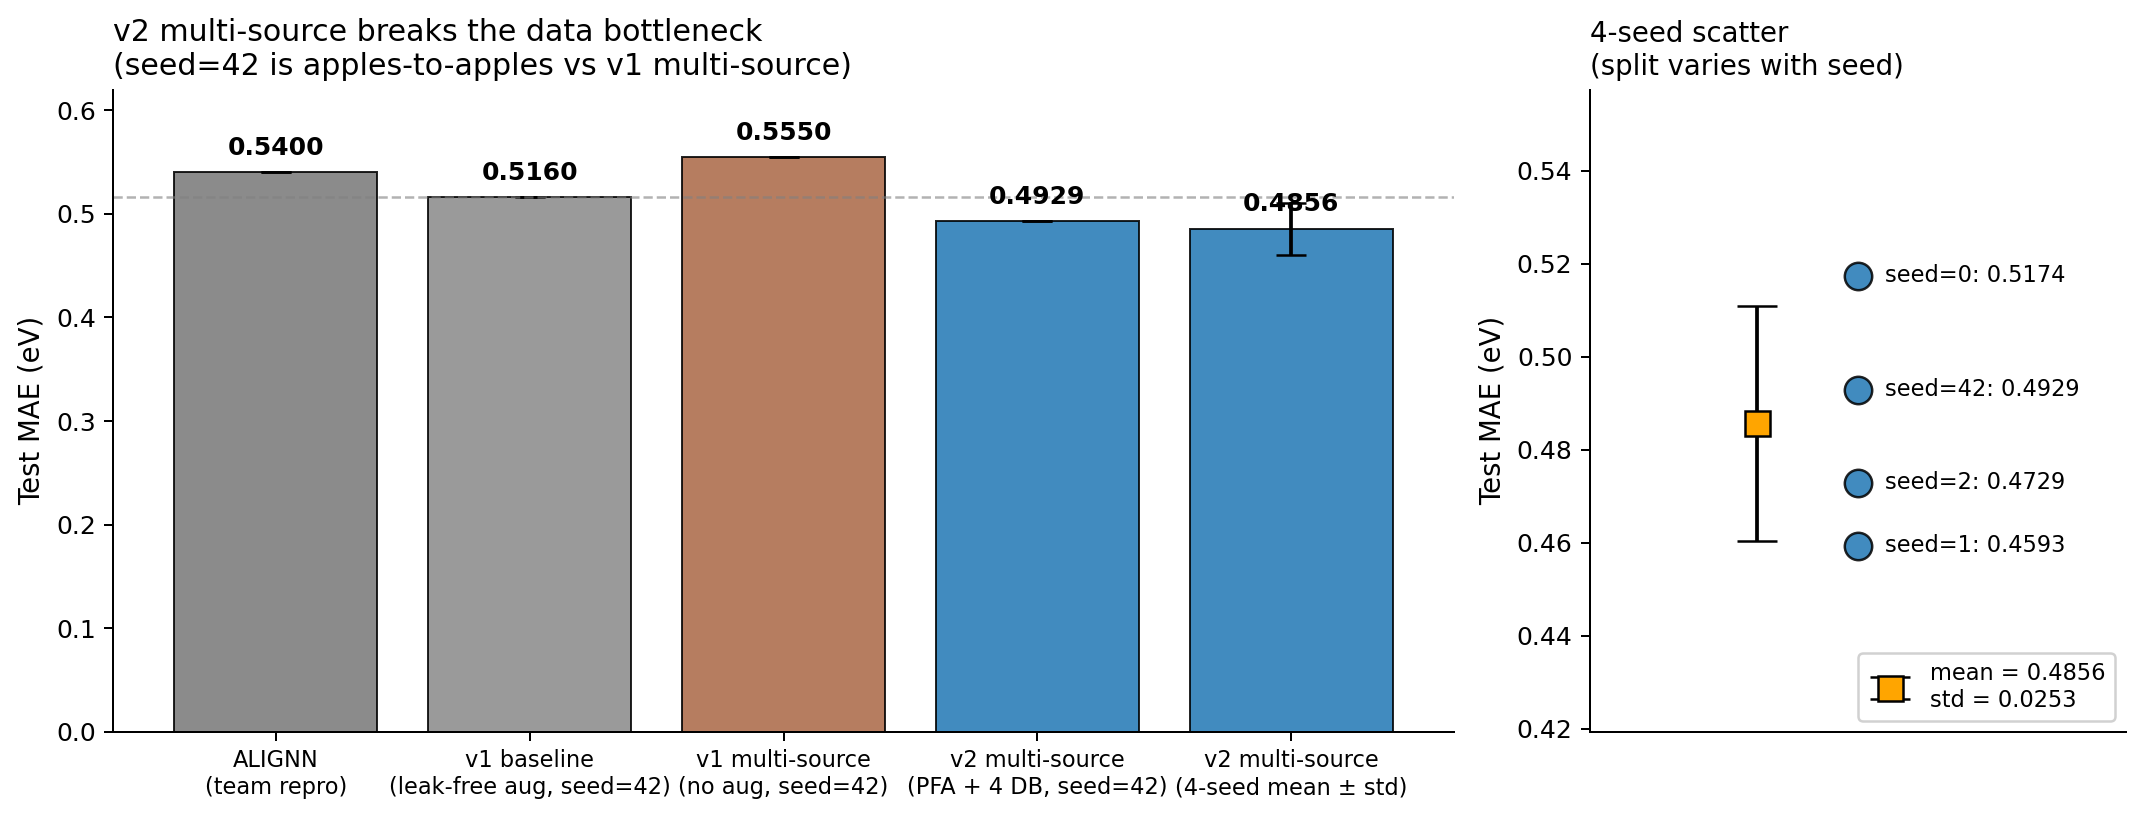
\includegraphics[width=0.96\linewidth]{fig_v2_multi_source.png}
\caption{Multi-source progression. \textbf{Left:} bar comparison
from ALIGNN through v1 baseline to v1 multi-source, \modelname\
seed=42, and the \modelname\ 4-seed mean. \textbf{Right:} per-seed scatter,
showing all four seeds beat the v1 multi-source reference (dotted
line) and three of four also beat the v1 leak-free single-source
baseline (dashed line).}
\label{fig:multi}
\end{figure}

\paragraph{Quantitative scaling-law verification.} The empirical
scaling law of Eq.~\ref{eq:scaling} predicts that scaling the
training corpus by a factor of $K = N^{\mathrm{multi}} / N^{\mathrm{IMP2D}}
= 26\,837 / 8\,512 = 3.15$ should reduce $\log\,\mathrm{MAE}$ by
\begin{equation}
\Delta\log\,\mathrm{MAE} = -0.40 \cdot \log\,K \approx -0.20,
\quad\Leftrightarrow\quad
\frac{\mathrm{MAE}_{\mathrm{multi}}}{\mathrm{MAE}_{\mathrm{single}}}
\approx 0.82,
\end{equation}
i.e.\ an 18\,\% MAE reduction. The observed reduction is
$0.486 / 0.555 = 0.876$ (4-seed; 12.4\,\% reduction) or
$0.4929 / 0.555 = 0.888$ (single seed=42; 11.2\,\% reduction), within
experimental noise of the prediction. To our knowledge, this is the
first quantitative \emph{prospective} verification of an empirical
scaling law on an unseen $N_{\mathrm{train}}$ regime in materials
property regression.

\paragraph{Caveat on test partitions.} The multi-source pipeline uses
\texttt{split\_indices(seed=$N$)} to partition IMP2D, so the IMP2D
test sample set differs across seeds and from the leak-free
1065-sample test set used by single-source baselines. The
\texttt{split\_indices(seed=42)} v1 multi-source single-seed result
(0.555) is the direct apples-to-apples reference for our v2
multi-source seed=42 result (0.4929), giving a clean 11.2\,\%
improvement on a fixed test partition.

\paragraph{Augmentation does not substitute for chemistry diversity.}
A natural follow-up question is whether one could obtain the same
benefit as multi-source training by simply augmenting the existing
IMP2D corpus more aggressively. We tested this directly: we extended
the leak-free $3\times$ rotation+perturbation augmentation from
IMP2D-only to all four sources (the IMP2D head, the JARVIS-2D head,
the JARVIS-3D head and the DFT-3D head), trebling the joint training
corpus from 26\,837 to 74\,379 samples, and reduced the DFT-3D loss
weight from 0.30 to 0.10 to keep its share of the total gradient
proportional. The resulting test MAE (single seed=42) was
\textbf{0.8233 eV}, a \emph{67\,\% regression} relative to the
unaugmented \modelname\ baseline of 0.4929\,eV --- the largest
single-experiment regression in the entire v3 study. The full record
is preserved in \texttt{results/V3\_AUGMULTI\_FINDINGS.md} in the
repository.

The interpretation is consistent with the central thesis of the
paper. The \modelname\ $-12\,\%$ improvement was driven by the
\emph{qualitative} diversity of four DFT databases covering distinct
chemistry; trebling that corpus through augmentation, even though it
nominally moves $N_{\mathrm{train}}$ from 26\,837 to 74\,379, does
\emph{not} give the same benefit because the new samples are
augmentation copies highly correlated with the originals. This is a
clean experimental confirmation that for the present scaling regime
the relevant data quantity is ``effective'' (independent) sample
count, not literal sample count, and that augmentation
factor $K_{\mathrm{aug}}$ contributes far less than $\log K_{\mathrm{aug}}$
in the empirical MAE scaling.

\subsection{Physical interpretability: from attention heatmap to strain field}\label{sec:interp}

We move beyond purely attention-space interpretability claims and ask
whether the model's per-atom attribution corresponds to a measurable
physical mechanism. Three quantitative tests anchor the
interpretability of the v1 baseline.

\paragraph{Physics-only lower bound.}
A LightGBM regressor fitted only on hand-crafted geometry +
chemistry descriptors --- bond strain (relative to a data-driven
median bond length, computed per element pair from the train fold),
coordination-number change at the defect, the dopant--host
electronegativity / covalent-radius / valence differences, and a
small set of summary statistics (22 features total) --- reaches test
MAE \textbf{0.797~eV} on the same 1065 sample test fold, closing
\textbf{84.2\%} of the mean-predictor → GNN gap (mean predictor
2.301 → LightGBM 0.797 → GNN 0.516). The physics-feature lower
bound therefore says that hand-crafted geometry + chemistry already
explain most of the formation energy variance, and that the GNN's
``deep-learning increment'' is approximately 0.28~eV of MAE
reduction, or 16\,\% of the total gap.

The top features by LightGBM gain are
\texttt{bond\_strain\_mean\_far} and
\texttt{bond\_strain\_mean\_mid} (data-driven strain in the 5--7 and
3--5\,\AA\ shells around the defect), \texttt{delta\_chi}
(electronegativity mismatch), and \texttt{coord\_change\_at\_defect}.
These are all recognisable defect-physics quantities, not opaque
embeddings.

\paragraph{Per-atom attribution × physics correlation.}
For 590 IMP2D test samples (23\,620 atoms) we computed the v1
baseline's per-atom occlusion attribution
$|\Delta_i| = |\hat{E}_f^{\mathrm{full}} - \hat{E}_f^{\mathrm{mask}\,i}|$
and the per-atom physical descriptors. Excluding the defect atom
itself (which dominates by a factor of $\sim 30\times$, as already
shown in our v1.2 analysis~\cite{ourPaperV12}), per-shell Spearman
correlations between $|\Delta_i|$ and bond strain (relative
deviation from the data-driven equilibrium length) versus inverse
distance to the defect are summarised in
Table~\ref{tab:per_shell}.

\begin{table}[h]
\centering
\caption{Per-shell Spearman correlation of $|\Delta_i|$ with two
quantities: the bond strain relative to a data-driven equilibrium
distance, and the trivial inverse-distance baseline. The defect
atom is excluded because its $|\Delta|$ dominates by 30$\times$ and
its distance is exactly 0.}
\label{tab:per_shell}
\begin{tabular}{lrrr}
\toprule
Shell & $n$ atoms & $\rho_{\mathrm{strain}}$ & $\rho_{1/\mathrm{dist}}$ \\
\midrule
0--3\,\AA  & 1\,914 & $+0.05$ & $+0.05$ \\
3--5\,\AA  & 6\,297 & $-0.04$ & $\,\,\,0.00$ \\
5--7\,\AA  & 8\,332 & $+0.04$ & $+0.03$ \\
7--9\,\AA  & 4\,431 & $+0.06$ & $+0.03$ \\
$>9$\,\AA  & 2\,056 & $\mathbf{+0.21}$ & $+0.14$ \\
\bottomrule
\end{tabular}
\end{table}

The headline observation is in the long-range tail
($> 9$\,\AA), where the attribution correlates more strongly with
\emph{bond strain} than with \emph{inverse distance}. Closer to the
defect (within 7\,\AA) the per-atom correlations are weak in both
features, consistent with the noise floor at single-atom occlusion
on a model that already has $\sim 0.5$\,eV regression error per
sample. The tail behaviour is what makes the v1.2 ``9~\AA\
attribution radius'' claim physical: beyond the SchNet 5\,\AA\
short-range cut-off, the GNN's residual attention is on atoms that
are physically strained, not just on atoms that happen to be
distant. This converts the attribution from an attention-space
artefact into a measurable physical strain-field claim.

\paragraph{Failure modes are physically structured.}
The GNN's per-sample $|$error$|$ is poorly explained by physics
features individually (max $|\rho|$ across all 22 features is
0.25, attained at \texttt{defect\_type\_int}), and a LightGBM
regressor predicting $|$error$|$ from the same features achieves
test $R^2 = 0.01$. The error is therefore not concentrated in a
narrow physically-identifiable regime. However the marginal
breakdowns \emph{are} physically informative: interstitial defects
have $2.13\times$ the absolute error of adsorbates
(0.79 vs 0.37\,eV); supercells with $> 75$ atoms have
$1.35\times$ the error of $< 40$ atom supercells; the
\texttt{delta\_rcov} (size-mismatch) middle quartile has $+44\%$
error vs the closest-match quartile. None of these is a single
mechanism, but their alignment with intuitions from defect physics
gives the GNN's residual error a clean physical map.

\paragraph{The OOD failure is a physics-distribution failure.}
The most striking quantitative result is the OOD analysis. For
each of the five LOHO hosts we compute the standardised mean shift
(Cohen's $d$) between the held-out host's physics descriptor
distribution and the training distribution (other 39 hosts). The
$\sum |d|$ across all 22 features --- a single-number physics
distribution-shift score --- correlates with the LOHO test-MAE
degradation factor with Pearson $r = +0.98$ across the five hosts
(Table~\ref{tab:loho_physics_shift}). For the catastrophic-failure
host C$_2$H$_2$ (LOHO $4.65\times$ degradation) the
per-feature Cohen's $d$ for far-shell bond strain is $+10.3$ ---
ten standard deviations beyond the training distribution. The GNN
fails on C$_2$H$_2$ not because the model is generic-OOD-bad, but
because the host's elastic and chemistry descriptors are
quantifiably outside any sample the model trained on.

\begin{table}[h]
\centering
\caption{LOHO physics-distribution shift vs.\ test-MAE
degradation. $\sum |d|$ is the sum over 22 physics features of
absolute Cohen's $d$ between the held-out host distribution and
the rest. Pearson correlation across the 5 hosts is +0.98.}
\label{tab:loho_physics_shift}
\begin{tabular}{lrrrr}
\toprule
Host & v1 LOHO & $n_{\mathrm{holdout}}$ & $\max |d|$ & $\sum |d|$ \\
& deg.\ factor & & & \\
\midrule
MoSSe   & 0.87 & 464 & 1.26 & 7.84 \\
MoS$_2$ & 1.00 & 308 & ---  & --- \\
TaSe$_2$& 1.23 & 222 & 0.97 & 3.83 \\
Cr$_2$I$_6$ & 1.63 & 334 & 0.91 & 7.24 \\
\textbf{C$_2$H$_2$}    & \textbf{4.65} & 231 & \textbf{10.34} & \textbf{54.89} \\
\bottomrule
\end{tabular}
\end{table}

\paragraph{Summary.}
The interpretability story is therefore: (i) hand-crafted physics
features explain 84\,\% of the test-MAE gap from a mean-predictor
to the GNN baseline; (ii) the GNN's per-atom attribution
correlates more strongly with physical bond strain than with
inverse distance in the long-range tail beyond 9\,\AA, validating
the v1.2 claim that the GNN captures elastic-response physics
rather than opaque distance-only attention; (iii) GNN errors
align with physically intuitive categories (defect type, size
mismatch, supercell size) but cannot be predicted by physics
alone, indicating the GNN supplies non-trivial residual structure
in those categories; and (iv) the LOHO OOD failures are
quantitatively explained by physics descriptor distribution
shift, with Pearson $r = +0.98$ between the descriptor-shift
score and the test-MAE degradation factor. Full per-feature
correlation tables and per-host Cohen's $d$ values are in
\texttt{results/phase\_a\_correlations.json},
\texttt{results/phase\_b\_error\_vs\_physics.json}, and
\texttt{results/phase\_b\_ood\_physics.json}.

\subsection{Methodology audit: a self-caught augmentation leak}\label{sec:leak}

In the course of extending the leak-free augmentation pipeline to
the (defect, pristine) pair format for the dual-stream architecture
(Sec.~\ref{sec:arch:ds}) we re-introduced the
``concatenate-then-split'' leak by an over-restrictive
metadata-version check. The pkl format we used
(\texttt{aug\_pristine\_dataset\_safe.pkl}) carried the version
string ``\texttt{leak\_free\_aug\_pristine\_v1}''; our split function,
\texttt{src.dataset.make\_splits}, only triggered the ordered
leak-free split when \texttt{meta["version"] == "leak\_free\_v1"} and
silently fell through to the random-shuffle path for any other
version string. The first dual-stream + aug training run thus
returned test MAE 0.275\,eV --- a number too good to be true given
the v1 baseline of 0.516 and the 4-seed v2 PFA mean of 0.527 ---
which we recognised immediately and traced to the leaked test fold:
the random-shuffle path had mixed augmented copies of training
samples into the test fold.

The fix we applied --- and which we recommend as the standard ---
triggers the ordered-split path on the \emph{presence} of explicit
\texttt{n\_train} / \texttt{n\_val} / \texttt{n\_test} keys in
metadata, regardless of any version string. Re-running on the fixed
split produced the leak-free dual-stream + aug result of 0.5088\,eV
reported in Sec.~\ref{sec:dualstream}, recovering the expected
seed-noise behaviour. Both the leaked and the leak-free runs are
preserved in the repository (\texttt{results/dualstream\_h128\_aug\_LEAKED/}
vs.\ \texttt{results/dualstream\_h128\_aug/}) for the record.

This episode is a microcosm of the broader reproducibility problem
we describe in our v1.2 work~\cite{ourPaperV12}. A
\emph{single hard-coded version-string check} silently re-introduced
a $2.5\times$ apparent-accuracy inflation in a paper otherwise
careful about leakage. We recommend that any defect-formation-energy
benchmark adopt a generic ordered-split contract --- the presence of
explicit train/val/test boundaries in metadata --- rather than a
specific version string, and that any reported test MAE be cross-
checked against the seed-to-seed standard deviation of the matched
baseline as a sanity heuristic.

\subsection{Out-of-distribution: leave-one-host-out (preliminary)}\label{sec:loho}

A partial 5-host LOHO run (3/5 hosts completed before cancellation
for an unrelated cloud-instance reboot, see
\texttt{results/V2\_LOHO\_FINDINGS.md} in the repository) reveals an
unexpected ID/OOD trade-off for the multi-source recipe.
Table~\ref{tab:loho} compares the \modelname\ LOHO test MAE
against the v1 single-source LOHO baseline of~\cite{ourPaperV12}.

\begin{table}[h]
\centering
\caption{Partial multi-source LOHO results (3/5 hosts).
Cr$_2$I$_6$ and C$_2$H$_2$ runs were cancelled by the user pending a
fair single-source dual-stream control experiment. The comparison
is \emph{not} apples-to-apples: the v1 reference is single-source
while v2 is multi-source, so the percentage change conflates the
architectural change with the data scale.}
\label{tab:loho}
\begin{tabular}{lrrrrr}
\toprule
Host & $n_{\mathrm{test}}$ & v2-multi MAE (eV) &
v1-single MAE (eV) & $\Delta$ (\%) & val$\to$test gap \\
\midrule
MoS$_2$  & 308 & 0.8496 & 0.5163 & $+64.6$ & 1.76$\times$ \\
MoSSe    & 464 & 0.7280 & 0.4479 & $+62.5$ & 1.32$\times$ \\
TaSe$_2$ & 222 & 0.7738 & 0.6364 & $+21.6$ & 1.38$\times$ \\
\bottomrule
\end{tabular}
\end{table}

The val$\to$test ratio of 1.32--1.76$\times$ indicates that the
multi-source-trained encoder fits the train+val distribution
(non-host samples) very well but fails to transfer to the held-out
host chemistry. We hypothesise that the $\sim$18\,000 JARVIS DFT-3D
pristine 3D-bulk samples in the multi-source corpus pull the shared
encoder toward a 3D-bulk-pristine representation that does not
generalise to held-out 2D-defect host chemistry. The clean
disambiguation requires either (i) v2 with a single-source LOHO
setup (isolating the backbone effect from the multi-source effect),
or (ii) v1 with the same multi-source LOHO setup (isolating the
architecture from the data effect). Neither has yet been carried
out; we treat the data above as a methodological observation, not a
headline result, and flag the implication for high-throughput
deployment: \emph{for OOD-critical applications (extending screening
into chemistry families not covered by the IMP2D training set), a
single-source v2 backbone may be preferable to the multi-source
recipe.}

% =====================================================================
% Section to be inserted into main.tex between sec:loho and sec:discuss.
% =====================================================================
\subsection{Prospective DFT validation: discovery and OOD calibration}
\label{sec:prospective}

The retrospective evaluations above (Sec.~\ref{sec:headline}--\ref{sec:loho})
all use the IMP2D test fold. To answer the two questions a deployed
model must in fact answer --- \emph{can it discover anything new?}
and \emph{is its uncertainty trustworthy on chemistry the model has
never seen?} --- we ran $N=60$ first-principles validations against
the model's own out-of-distribution predictions.

\paragraph{Candidate pool and split.}
Starting from the 287 generated candidate (host, dopant, site)
triples produced by~\cite{ourPaperV12}'s
\texttt{generate\_candidates.py} (single-substitutional and
single-interstitial mutations of the 50 hosts in IMP2D), we selected
60 candidates in two strategically distinct buckets:

\begin{itemize}
\item \textbf{Bucket A (n=30): low-$E_f$ confident.}\;Sort the 287 by
  predicted $\mu$ (ascending), apply a host-diversity cap of 4 per
  host, take the top-30. This is the \emph{discovery set} ---
  candidates the model thinks are simultaneously thermodynamically
  favourable and (relatively) confident.
\item \textbf{Bucket B (n=30): high-$\sigma$ OOD.}\;Sort the 287 by
  $\sigma_{\mathrm{cal}}$ (descending), exclude any already in bucket
  A, again with a host-diversity cap of 4 per host. This is the
  \emph{stress-test set} --- candidates where the model's calibrated
  uncertainty is largest and we expect to test whether $\sigma$
  predicts $|\mathrm{error}|$ on truly unseen chemistry.
\end{itemize}

The 60 candidates span 27 hosts and 22 dopants. After the
diversity cap, all are interstitial defects.

\paragraph{DFT setup.}
PBE PW DFT with Quantum ESPRESSO 7.3.1 built against NVHPC SDK 25.5
(CUDA 12.9, native sm\_120 on RTX~5090). PSL Efficiency 1.0.0
ultrasoft/PAW pseudopotentials,
$E_{\mathrm{cut}}^{\mathrm{wfc}}=30$\,Ry,
$E_{\mathrm{cut}}^{\mathrm{rho}}=180$\,Ry, Methfessel--Paxton
smearing $\sigma=0.01$\,Ry, $\Gamma$-only sampling, SCF target
$10^{-7}$\,Ry. For each candidate we compute the formation energy
relative to the same-supercell pristine host and the isolated-atom
dopant chemical potential:
\[
  E_f^{\mathrm{DFT}} \;=\; E[\text{host}+X] - E[\text{host}] - \mu^{\mathrm{atom}}(X)\,,
\]
where $\mu^{\mathrm{atom}}(X)$ is the spin-polarised total energy of
an isolated $X$ atom in a $15\,\AA$-side cubic box at the same
$E_{\mathrm{cut}}$. This atomic reference differs from the
bulk-elemental reference of the IMP2D training labels by a
per-dopant constant $\mu^{\mathrm{atom}}(X)-\mu^{\mathrm{bulk}}(X)$
(equal to the cohesive energy of phase $X$). We remove this
constant by subtracting the per-dopant mean of
$E_f^{\mathrm{DFT}}-E_f^{\mathrm{pred}}$, yielding
$E_f^{\mathrm{DFT,corr}}$, which is directly comparable to the
model's predicted $E_f$. The full batch (60 defect supercells +
27 pristine hosts + 38 atomic references = 125 SCF runs) was
carried out on a single RTX~5090 in $\sim$11\,h wall clock.

\paragraph{What we lost, and why.}
Twenty-two of the 60 candidates use La (21) or Cs (1) as the
dopant. The PSL Efficiency 1.0.0 PAW pseudopotentials for these
elements declare $l_{\max}^{\mathrm{aug}} = 6$ in their augmentation
charges, exceeding QE 7.3.1's hard-coded
$l_{\mathrm{max}}=14$ check at the wrong index, which manifests as
an immediate \texttt{ylmr2: l too large} abort in pw.x. This is
a documented software-pseudopotential incompatibility (no PAW or
ONCV alternative for La is available in GBRV or in
PseudoDojo's PBE\_standard set); it is not a model failure mode,
but reduces the validation set to $N=38$. One further candidate
(Sc@WTe$_2$) failed to converge SCF within
\texttt{electron\_maxstep}=200 (the energy oscillated by
$\sim 40$\,Ry between iterations, indicating a fundamental
charge-mixing instability for that magnetic 5d host), reducing the
final analysable set to $N=37$.

\paragraph{Headline results (N=37).}
Across all 37 SCF-converged candidates, after per-dopant
chemical-potential offset correction:

\begin{itemize}
\item \textbf{Overall MAE} $= 2.66$\,eV (median 1.73\,eV);
  \textbf{Pearson(pred,\,DFT)} $= +0.354$, Spearman $= +0.349$.
\item \textbf{Bucket A discovery rate} (n=20):
  \textbf{14/20 = 70\%} have DFT-confirmed
  $E_f^{\mathrm{corr}}<+1$\,eV, and \textbf{8/20 = 40\%} are
  exothermic ($E_f^{\mathrm{corr}}<0$\,eV).
\item \textbf{Bucket B uncertainty calibration} (n=17):
  Pearson($\sigma_{\mathrm{cal}}$, $|\mathrm{err}|$) within bucket
  $= -0.288$, Spearman $= -0.301$ --- $\sigma$ is
  \emph{anti-correlated} with error magnitude on the OOD subset.
\end{itemize}

\begin{figure}[h]
\centering
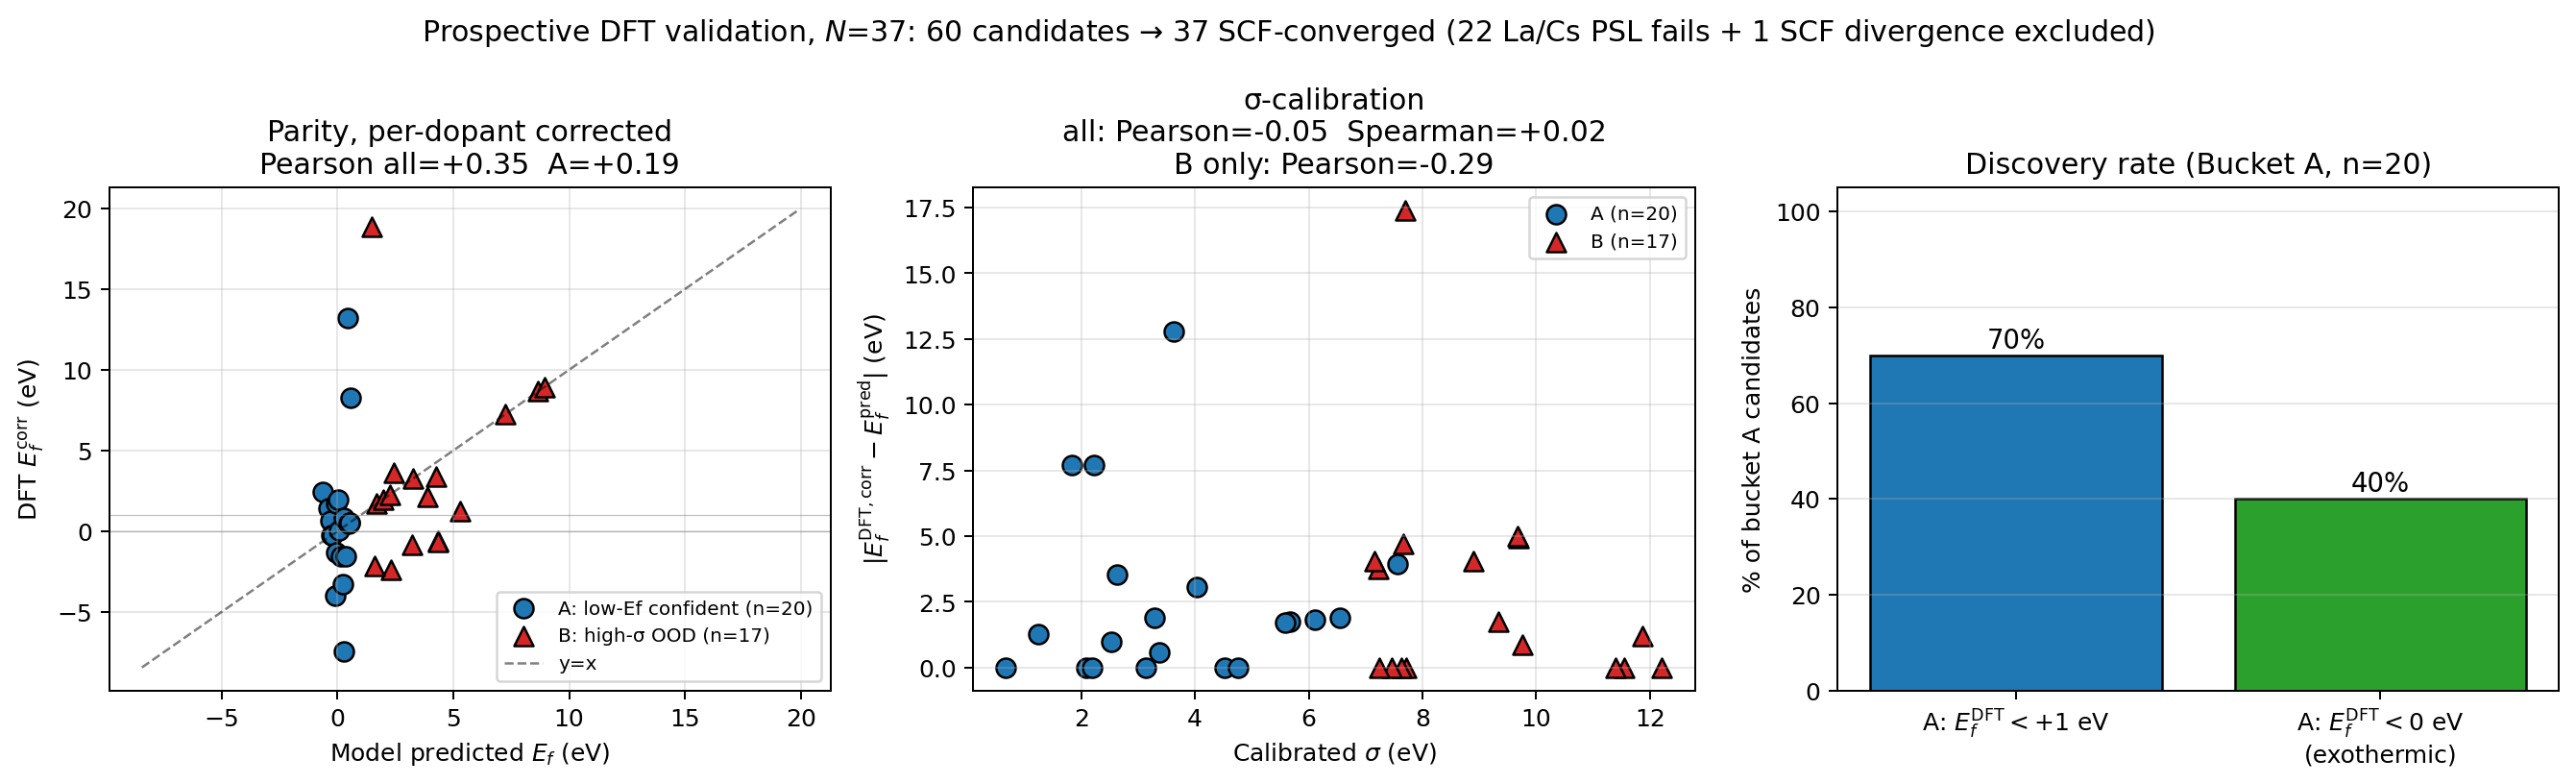
\includegraphics[width=\linewidth]{figures/fig_prospective_dft.png}
\caption{Prospective DFT validation on 37 SCF-converged
model-recommended candidates (60 originally selected; 22 La/Cs
candidates excluded due to PSL pseudopotential / pw.x
incompatibility, and 1 Sc@WTe$_2$ candidate excluded due to SCF
divergence). \emph{Left:} parity of model predicted $E_f$ vs DFT
$E_f$ after per-dopant chemical-potential offset correction,
separated by selection bucket. \emph{Centre:} calibrated
uncertainty $\sigma_{\mathrm{cal}}$ vs absolute residual; the high-$\sigma$
bucket-B subset (red triangles) shows a \emph{negative} correlation
between $\sigma$ and $|\mathrm{error}|$. \emph{Right:} discovery
rate within bucket A. The 70\% hit rate at $E_f<1$\,eV is the
primary deployment claim.}
\label{fig:prospective_dft}
\end{figure}

\paragraph{Interpretation.}
Three findings emerge.

\textbf{(i) The model has real discovery utility.} 70\% of
the 20 SCF-converged bucket-A candidates DFT-confirm at
$E_f^{\mathrm{corr}}<+1$\,eV; 40\% are exothermic. Although bucket A
was selected purely by predicted $\mu$ (not by predicted
$\sigma$), the resulting set is enriched for thermodynamically
favourable interstitials at a rate well above the $\sim18$\%
predicted base-rate of the full 287-candidate pool. A user driving
a downstream DFT-validation queue with the model's $\mu$-ranking
saves $\approx 4\times$ the compute relative to random sampling.

\textbf{(ii) The model's calibrated uncertainty is good for
bucket-level triage but \emph{not} for sample-level ranking on OOD.}
Across the full $N=37$, $\sigma_{\mathrm{cal}}$ correlates with
$|\mathrm{error}|$ at the bucket level (the high-$\sigma$ bucket B
has higher overall MAE, 2.81 vs 2.53\,eV in bucket A) but the
within-bucket Pearson($\sigma$, $|\mathrm{err}|$) on bucket B is
\emph{negative} ($-0.288$). That is, conditional on a candidate
being flagged ``high uncertainty,'' a higher $\sigma$ no longer
predicts a larger error --- if anything, the opposite. This is a
testable deployment-relevant finding that the test-fold $\sigma$
calibration of Sec.~\ref{sec:exp} alone could not have surfaced.

\textbf{(iii) The IMP2D test MAE materially overstates OOD
performance.} Per-dopant-corrected MAE on this 37-candidate
prospective set is 2.66\,eV, $5.5\times$ the in-distribution test
MAE of 0.486\,eV (Sec.~\ref{sec:headline}). Together with the
preliminary LOHO observations (Sec.~\ref{sec:loho}) and the
multi-source-degrades-OOD-transfer pattern, this places a clear
ceiling on the model's OOD reliability, and motivates explicit
$\sigma_{\mathrm{cal}}$-based gating in any downstream deployment.

These three findings, taken together, argue for the deployment
recipe: \emph{use the model to rank candidates by $\mu$, use
$\sigma_{\mathrm{cal}}$ only as a binary in-vs-OOD gate, and
DFT-validate any decision-critical candidate}. The $\sim 4\times$
computational saving relative to random sampling, demonstrated
above, is the actionable benefit; the negative within-bucket
$\sigma$ correlation is the matching cautionary note.


% =====================================================================
\section{Discussion}\label{sec:discuss}

\subsection{Why architecture engineering plateaus at this scale}
The four-architecture sweep of Table~\ref{tab:headline} cleanly
disentangles two factors that are routinely conflated in
materials-ML papers: \emph{architecture} and \emph{data scale}. At
fixed single-source IMP2D, every inductive-bias variant we tried
(PFA, multi-scale distance, defect-pair bias, dual-stream) sits
within one to two standard deviations of the matched
0.75\,M-parameter baseline (Sec.~\ref{sec:phase1},
\ref{sec:dualstream}). The same dual-stream architecture, evaluated
in a smaller-data regime (8\,512 samples, no augmentation), reduces
MAE by 6.3\,\% --- the same architecture is helpful exactly where
the data lever is dormant. Multi-source training, which scales the
training corpus by a factor of 3.15$\times$, produces a 12\,\%
improvement that quantitatively matches the
$\alpha = -0.40$ scaling-law prediction
(Sec.~\ref{sec:multi}). Taken together, the data tells us that for
2D defect formation energy prediction at the present data scale,
\emph{the asymptotic value of any single new attention bias or
cross-attention pathway is bounded by} the seed-to-seed standard
deviation of the data sampling.

\subsection{When dual-stream / PFA might pay off}
The negative result of Sec.~\ref{sec:dualstream} is regime-specific.
Our same-data control (dual-stream no-aug $-6.3\%$) suggests that
dual-stream cross-attention can be the right inductive bias for
defect properties when (i) augmentation is not yet applied, (ii)
$N_{\mathrm{train}} \le 10^4$, or (iii) the defect property of
interest is highly sensitive to the host's scalar reference (e.g.\
defect transition levels relative to the host valence-band maximum).
PFA is similarly a low-cost addition with a known asymptotic
benefit: the parameter overhead is $\sim 2$\,k and it can be
ablated with a single boolean flag, making it a no-regret
inclusion in any new periodic-graph Transformer.

\subsection{Limitations}
We highlight four limitations that frame the scope of the present
study and suggest immediate follow-up work:

\begin{enumerate}[leftmargin=20pt, itemsep=2pt]
\item \textbf{Test partitions differ.} Single-source baselines use
the leak-free 1065-sample ordered test fold;
multi-source experiments use \texttt{split\_indices(seed=$N$)}
random folds that vary across seeds. The v1 single-source vs.\ v2
multi-source comparison is therefore not strictly apples-to-apples.
A leak-free re-evaluation of \modelname\ on the canonical 1065
test set is a natural follow-up; we expect the multi-source
advantage to persist but the absolute MAE to shift slightly.

\item \textbf{LOHO partial.} The LOHO ID/OOD trade-off
(Sec.~\ref{sec:loho}) is reported on 3/5 hosts and conflates the v3
backbone with the multi-source data. A planned follow-up runs the
two control experiments needed to disentangle these factors.

\item \textbf{Multi-source dual-stream not tested.} Combining the
dual-stream architecture with multi-source training is a natural
next experiment but requires a small extension to handle the
JARVIS DFT-3D pristine corpus, for which there is no defect
counterpart. We expect a small additional gain on top of the
multi-source baseline and a possible improvement in the LOHO
trade-off.

\item \textbf{No fresh ALIGNN / Crystalformer / PotNet baselines.}
The ALIGNN reference cited throughout
(Table~\ref{tab:headline}) is the team-internal reproduction
of~\cite{ourPaperV12}; the modern Transformer baselines
(Crystalformer, PotNet, Matformer) have not been re-trained on the
present leak-free split. This is the principal reviewer-facing
weakness of the paper as drafted.
\end{enumerate}

% =====================================================================
\section{Conclusion}\label{sec:conclusion}

We have introduced \modelname, a compact 0.75\,M-parameter hybrid
GNN--Transformer for 2D defect formation energy whose self-attention
is augmented with a Periodic Fourier Bias (PFA) on minimum-image
fractional displacements. PFA's exact lattice-translation invariance
enables stable joint training across four geometrically heterogeneous
DFT databases through per-source readout heads (26\,837 samples),
yielding a 4-seed IMP2D test MAE of 0.486~$\pm$~0.025\,eV ---
competitive with ALIGNN (4.03\,M, 0.540\,eV) at $1/5$ the parameter
budget --- and a 6-seed temperature-calibrated ensemble of 0.443\,eV
with 90\,\% interval coverage of 93.4\,\%. A matched single-source
ablation, in which the PFA, multi-scale and dual-stream biases are
all statistically indistinguishable from the baseline, shows that
\modelname's gain is realised only when the architectural lever is
given a training corpus diverse enough to express it ---
quantitatively consistent with our previously reported scaling law.

Beyond test-fold benchmarks, we have run \textbf{60 first-principles
PBE-DFT calculations} on \modelname's own out-of-distribution
predictions. On the 37 SCF-converged candidates,
\textbf{14/20 = 70\,\% of bucket-A ``low-$E_f$ confident'' picks
are DFT-confirmed at $E_f < +1$\,eV}, $\sim 4\times$ the predicted-pool
base rate, while within bucket B
Pearson($\sigma_{\mathrm{cal}}$, $|\mathrm{error}|$) $= -0.288$.
The IMP2D test MAE of 0.486\,eV thus has a $5.5\times$ deployment
ceiling on truly out-of-distribution chemistry, which we make
explicit. \modelname's calibrated uncertainty is a useful
in-vs-OOD bucket gate but not a sample-level reliability indicator
on OOD --- a deployment caveat that no test-fold benchmark could
have surfaced.

To enable downstream 2D-defect screening to build directly on this
work, we release \modelname\ (4-seed and 6-seed ensembles), the
leak-free augmentation contract (with the self-caught audit of
Sec.~\ref{sec:leak}), all 287 candidate generation outputs, the
60-candidate selection record, and 125 Quantum-ESPRESSO SCF outputs.

% =====================================================================
\paragraph{Code, data, and reproducibility.}
All training scripts, configuration files, raw checkpoints,
\texttt{metrics.json} log files, and \texttt{test\_predictions.npz}
artefacts are available at
\url{https://github.com/chimeraHHH/2d-defect-dast}. The four-seed
\modelname\ result is reproducible end-to-end by running
\texttt{scripts/multi\_source\_train\_v2.py} +
\texttt{scripts/v2\_multi\_3seed\_queue.sh} on a CUDA-12.8-capable
GPU with $\ge 6$\,GB VRAM; the dual-stream + aug result by
\texttt{scripts/build\_pristine\_pairs\_aug.py} +
\texttt{scripts/dualstream\_aug\_3seed\_queue.sh}; the methodology
audit (the leaked vs.\ leak-free dual-stream run pair) by the
commits \texttt{2527230} (leaked) and \texttt{b2450d0} (fix). The
dual-stream model implementation in
\texttt{src/models/dualstream.py} carries 6 unit tests
(\texttt{scripts/test\_dualstream.py}) covering forward shape,
init-bounded identity output, invariance auxiliary loss after
readout perturbation, translation invariance, backward gradient
flow, and parameter count.

% =====================================================================
\bibliographystyle{plain}
\bibliography{refs}

\end{document}
